\chapter{Bounds from \texorpdfstring{$\mu^-$}{muon} decays}
\label{ch:MuBounds}
As was shown in the previous section, Michel parameters are linear combinations of coupling strengths of effective four point interactions that lead to the muon decay. Any three body decay that has a valid representation as this effective coupling then be calculated and expressed as a deviation from the known standard model values. This has long been used to restrict any additional interaction that might contribute to the decay. 

One path that has not been investigated beyond the change in the decay width however is the influence of another four body decay of the muon besides the radiative decay. If the muon decays to $e^-\bar{\nu}_e \nu_\mu X$ where $X$ is either a scalar $\phi$ or a dark photon $A'$, this would alter the decay spectrum but still register as a three body decay, as long as $X$ leaves the detector undetected or decays invisibly. The obvious standard model background is the radiative decay, where the photon is not detected. This nevertheless will alter the experimentally taken spectrum and in turn the determined Michel parameters. As an example this is shown in figure \ref{fg:MuonBSMContribution} where the dark photon couples to the electron and electron neutrino.
\begin{figure}[ht]
\centering
\begin{subfigure}{.5\textwidth}
  \begin{tikzpicture}
\begin{feynman}
\vertex (a) {\(\mu^{-}\)};
\vertex [right=of a] (b);
\vertex [above right=of b] (f1){\(\nu_\mu \)};
\vertex [below right=of b] (c);
\vertex [above right=of c] (d);
\vertex [above right=of d] (f2){\(e^-\)};
\vertex [below right=of d] (f4){\(A'\)};
\vertex [below right=of c] (f3){\(\bar{\nu}_e\)};
\diagram* {
(a)--[fermion](b)--[fermion](f1),
(b)--[boson, edge label'=\(W\)](c),
(d)--[boson](f4),
(f2)--[anti fermion](d)--[anti fermion](c)--[anti fermion](f3)};
\end{feynman}
\end{tikzpicture}
\end{subfigure}%
\begin{subfigure}{.5\textwidth}
\begin{tikzpicture}
\begin{feynman}
\vertex (a) {\(\mu^{-}\)};
\vertex [right=of a] (b);
\vertex [above right=of b] (f1){\(\nu_\mu \)};
\vertex [below right=of b] (c);
\vertex [above right=of c] (f2){\(e^-\)};
\vertex [below right=of c] (d);
\vertex [above right=of d] (f4){\(A'\)};
\vertex [below right=of d] (f3){\(\bar{\nu}_e\)};
\diagram* {
(a)--[fermion](b)--[fermion](f1),
(b)--[boson, edge label'=\(W\)](c),
(d)--[boson](f4),
(f2)--[anti fermion](c)--[anti fermion](d)--[anti fermion](f3)};
\end{feynman}
\end{tikzpicture}
\end{subfigure}
\caption{Example diagrams that result from a coupling between the dark photon and the electron/electron neutrino }
\label{fg:MuonBSMContribution}
\end{figure}
Since this cant be expressed as a four point interaction, there is not simple expression for the altered parameters. Another fact, that complicate things is there not much hope for a analytical solution for the phase space integral. So a numerical integration procedure is needed. 
\section{Calculation of the spectrum}
This case is less restricted than the pion decay, because here we deal with both electrons and muons.
The models that are investigated are a scalar coupling to the electron, the muon and both at the same time. The spin 1 model will couple to both the charged leptons as well as the neutrinos. For this case the coupling to the electron and muon are separately tested as well as combined. Additionally to this also the coupling to the left and right chiral fields are probed independently. 
The experimental values were obtained with $\sim 3\cdot 10^{9}$ muons. If one were to probe the BSM-models with Monte-Carlo event generators one would need BSM events of the order of $10^7$ to reach comparable or even better sensitivity and to be able to probe large coupling constants.
This takes long and generated a huge amount of data because even at later stages ignored information is generated and stored. 
This is why a custom numerical integration method was used. 

The squared matrix element for the polarised decay was traced and simplified in \textsc{Mathematica} by using the \textsc{Feyncalc}. The momenta were assigned according to equation \ref{eq:momenta} shown in the appendix. This in then parsed to C++ code to be integrated numerically. The phase space integral can be done by some quadrature method with weights $w_i$ and nodes $x_i$. This reduces the integration to the sums shown in equation \ref{eq:sum}.
\begin{equation}
\sum_{i_1=1}^{N(E_1)} \sum_{i_2=1}^{N(E_2)} \sum_{i_3=1}^{N(\theta_1)}  \sum_{i_4=1}^{N(\theta_2)}  \sum_{i_5=1}^{N(\theta_3)}  \sum_{i_6=1}^{N(\phi_2)}  \sum_{i_7=1}^{N(\phi_3)} w_{i_1}w_{i_2}w_{i_3}w_{i_4}w_{i_5}w_{i_6}w_{i_7}I(x_{i_1}...x_{i_7})
\label{eq:sum}
\end{equation}
To reach a sensible precision of less than one percent on the total decay width, the total order of nodes is of the order of $10^{10}$. Because the calculation is easily parallelised this can be done on a GPU in a matter of 3 hours for each model with the \textsc{CUDA} framework. All sums are carried out up to the $E_1$ and $\theta_1$ which are instead saved to a file.
Examples of these spectra are shown in figure \ref{fg:exampleSpectra}.
\begin{figure}[H]
\centering
\begin{subfigure}{.45\textwidth}
  \centering
  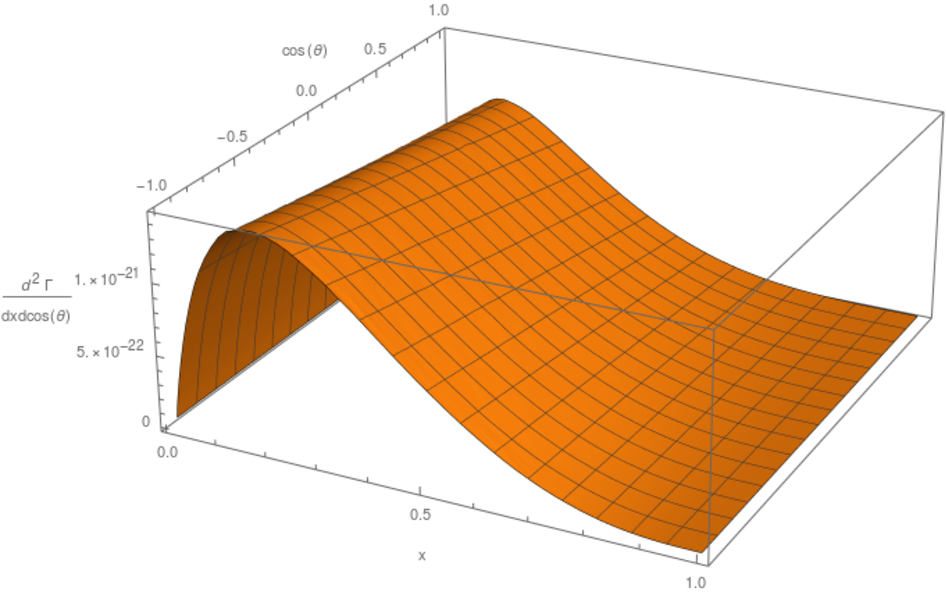
\includegraphics[width=\linewidth]{imgs/ScalarElectronPlot}
  \caption{Spectrum with $m_\phi=\SI{10}{\mega \eV}$ and coupling to the electron}
  \label{fg:ScaElSpectrum}
\end{subfigure}%
\begin{subfigure}{.45\textwidth}
  \centering
  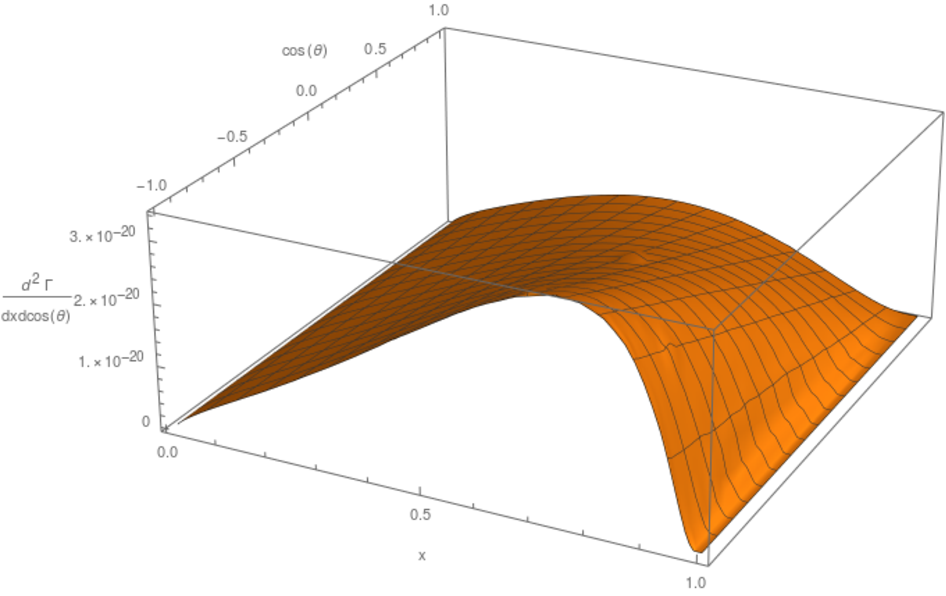
\includegraphics[width=\linewidth]{imgs/VectorLeptonPlot}
  \caption{Spectrum with $m_{A'}=\SI{10}{\mega \eV}$ and $L_e-L_\mu$ couplings}
  \label{fg:VecLepSpectrum}
\end{subfigure}
\caption{Example spectra}
\label{fg:exampleSpectra}
\end{figure}
\section{Validity checks}
The resulting spectrum need to be checked for validity to determine, whether the number of nodes is enough to resolve the structure of the integrand. First, for each scenario the remaining two sums are carried out to get the total decay width. This is then compared to the decay width as calculated by the tool \textsc{Calc-HEP} that is configured such that the estimated error is less than one part per thousand. Then both widths are compared. For $(N(E_1),N(E_1),N(\theta_1),N(\theta_2),N(\theta_3),N(\phi_1),N(\phi_2)=(60,60,60,25,25,25,25)$ both width easily agree. 
\section{Michel parameter extraction}
The spectra have been calculated with all BSM coupling constants set to unity. Now the known standard model decay spectrum from equation \ref{eq:Diffrate} is added to the BSM-spectrum that has been scaled by a factor $g^2$. This is then subject to a similar fitting routine as the experimentalists used to extract the values for $\rho$, $\delta$ and $\xi$. The overall scale factor in the experimental setup would be fixed by the total number of included events. Here the combination of both decay widths replaces this.
$g^2$ is then varied and the bisection method is used to find its maximum value that violates one or more of the expected values by $2\sigma$.
Then $g$ can be used as a bound on the BSM-coupling.
\section{Influence of the fiducial region}
The authors of \cite{TWIST:2011aa} had to restrict the part of the spectrum that was used to extract the Michel parameters because of the detector geometry and inefficiencies. The region used is shown in figure \ref{fg:FiducialRegion}. If the BSM-spectrum was concentrated outside the fiducial region, its influence would be greatly underestimated. To get comparable results, either the same region has to be used or the influence has to be tested as to make sure it can be neglected. 
\begin{figure}[ht]
  \centering
    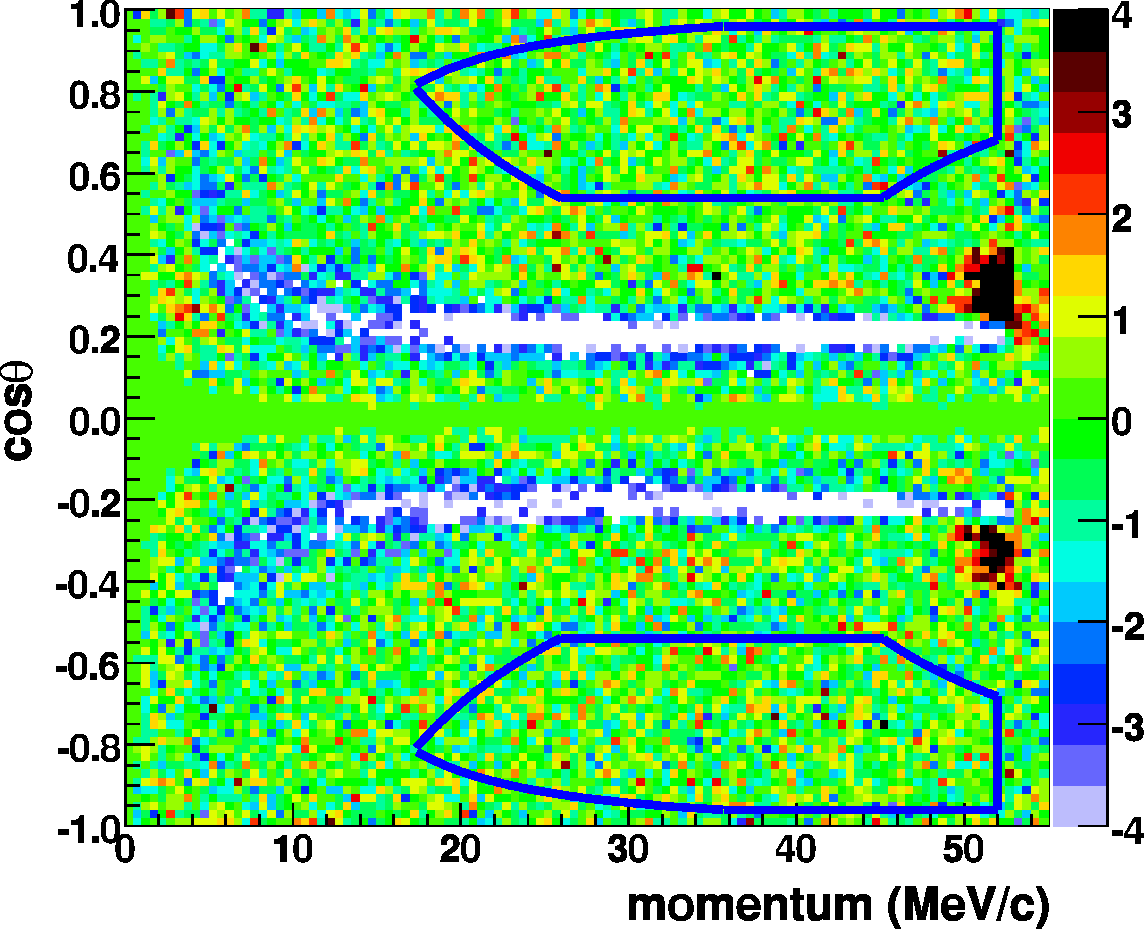
\includegraphics[width=0.6\textwidth]{imgs/fiducial}
    \caption{Fiducial region (blue) used by \cite{TWIST:2011aa}}
    \label{fg:FiducialRegion}
\end{figure}
Figure \ref{fg:MassDependence} shows the form of the spectra depending on the mediator mass. Clearly the bulk of the spectrum is included in the fiducial region, so that the experimental setup isn't accidentally blind to these processes. Only the heaviest mediators with masses $\geq \SI{50}{\mega \eV}$ avoids the active region. But the corresponding bounds are weak anyway because of the small width and are not competitive with existing bounds. 
The restriction to these regions worsens the bound only by a factor of order one where for almost all mass choices the bounds get weaker by a factor between two and four.
\begin{figure}[H]
	\centering
	\begin{subfigure}[b]{0.45\textwidth}
    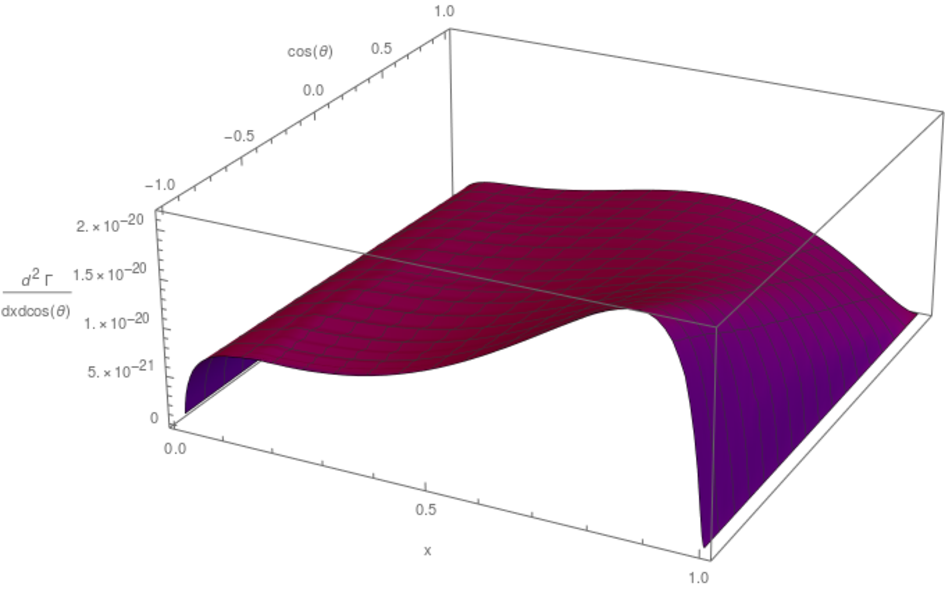
\includegraphics[width=\textwidth]{imgs/S0-001}
    \caption{$m_\phi = 1$MeV}
    \end{subfigure}
    ~
    \begin{subfigure}[b]{0.45\textwidth}
    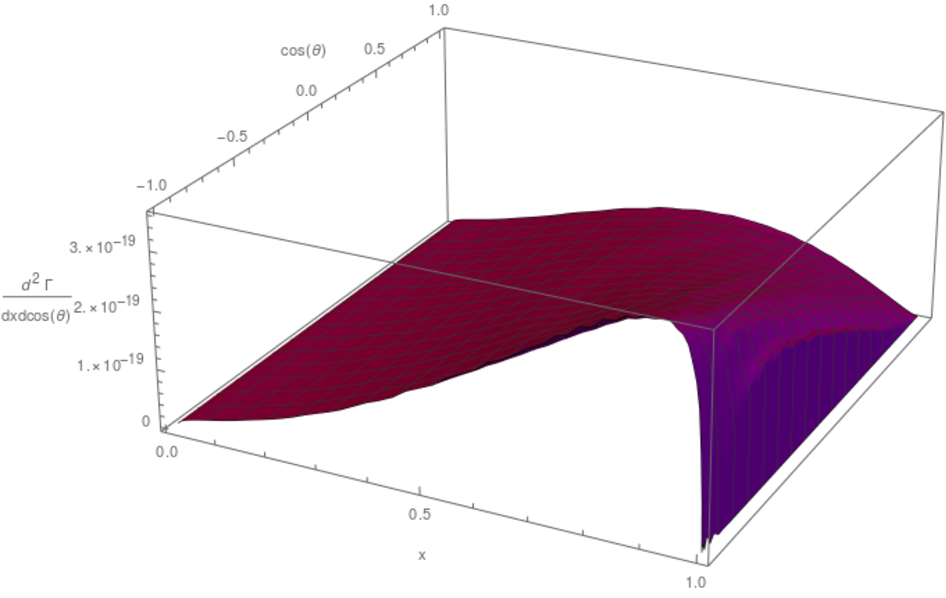
\includegraphics[width=\textwidth]{imgs/V0-001}
    \caption{$m_{A'} = 1$MeV}
    \end{subfigure}
    
    \begin{subfigure}[b]{0.45\textwidth}
    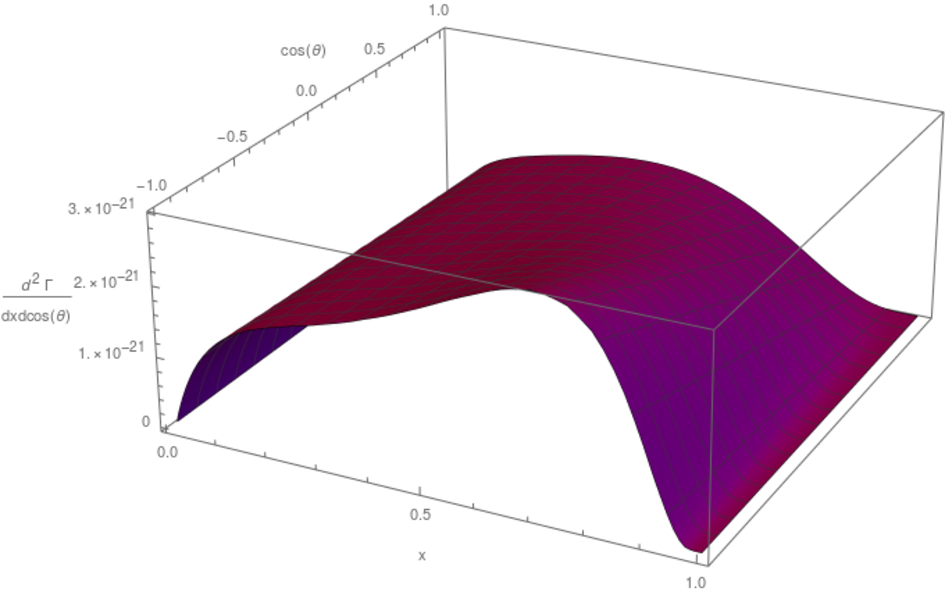
\includegraphics[width=\textwidth]{imgs/S0-01}
    \caption{$m_\phi = 10$MeV}
    \end{subfigure}
    ~
    \begin{subfigure}[b]{0.45\textwidth}
    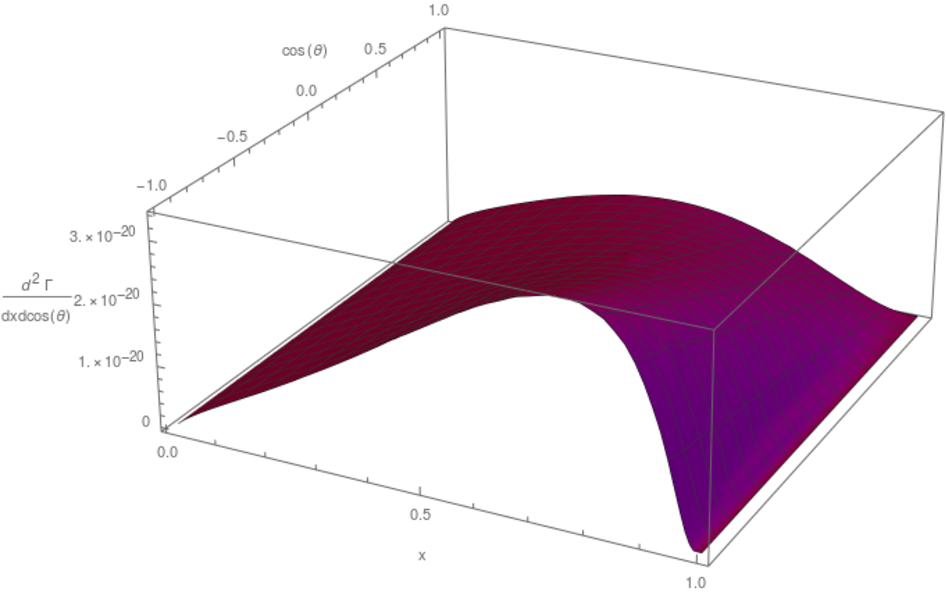
\includegraphics[width=\textwidth]{imgs/V0-01}
    \caption{$m_{A'} = 10$MeV}
    \end{subfigure}
    
    \begin{subfigure}[b]{0.45\textwidth}
    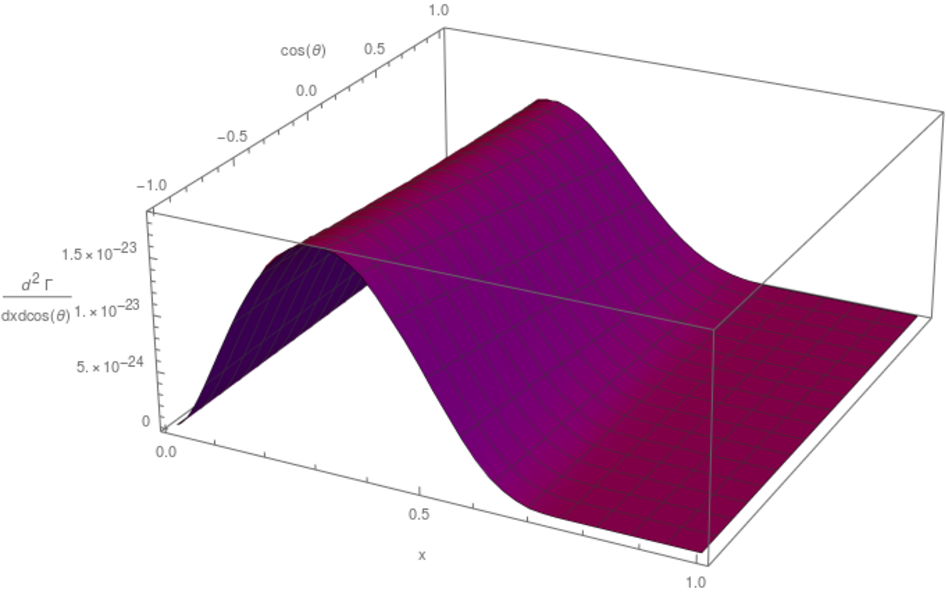
\includegraphics[width=\textwidth]{imgs/S0-05}
    \caption{$m_\phi = 50$MeV}
    \end{subfigure}
    ~
    \begin{subfigure}[b]{0.45\textwidth}
    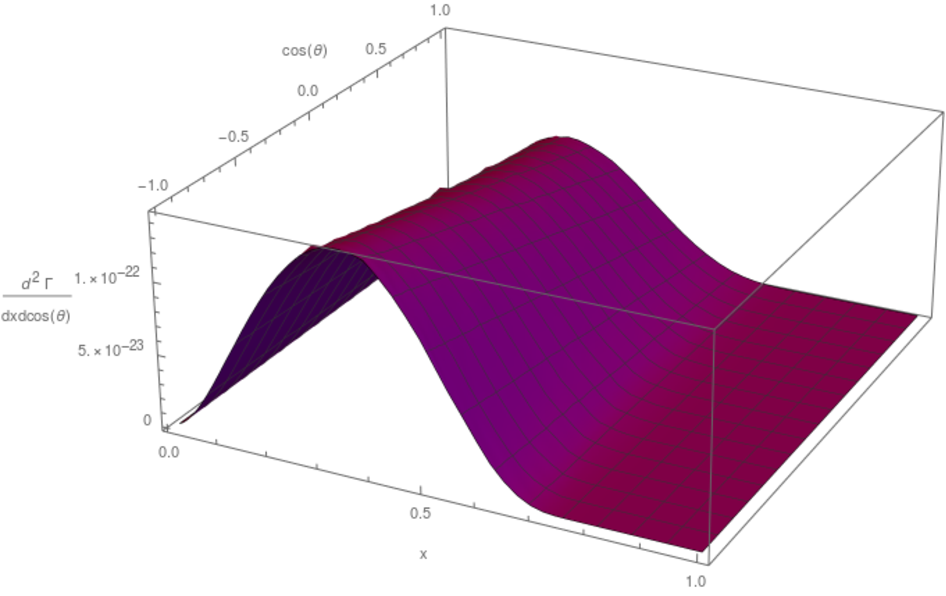
\includegraphics[width=\textwidth]{imgs/V0-05}
    \caption{$m_{A'} = 50$MeV}
    \end{subfigure}
    \caption{Scalar (left) and vector (right) mass dependence of the spectra}
    \label{fg:MassDependence}
\end{figure}
\newpage
\section{Results}
Here the resulting bounds on the couplings will be presented and compared to existing constraints. Because the existing literature doesn't use consistently either 90 \% or 95\% C.L. exclusions, both are shown in each graph. 
\subsection{Scalar Mediator}

\begin{figure}[!ht]
  \centering
    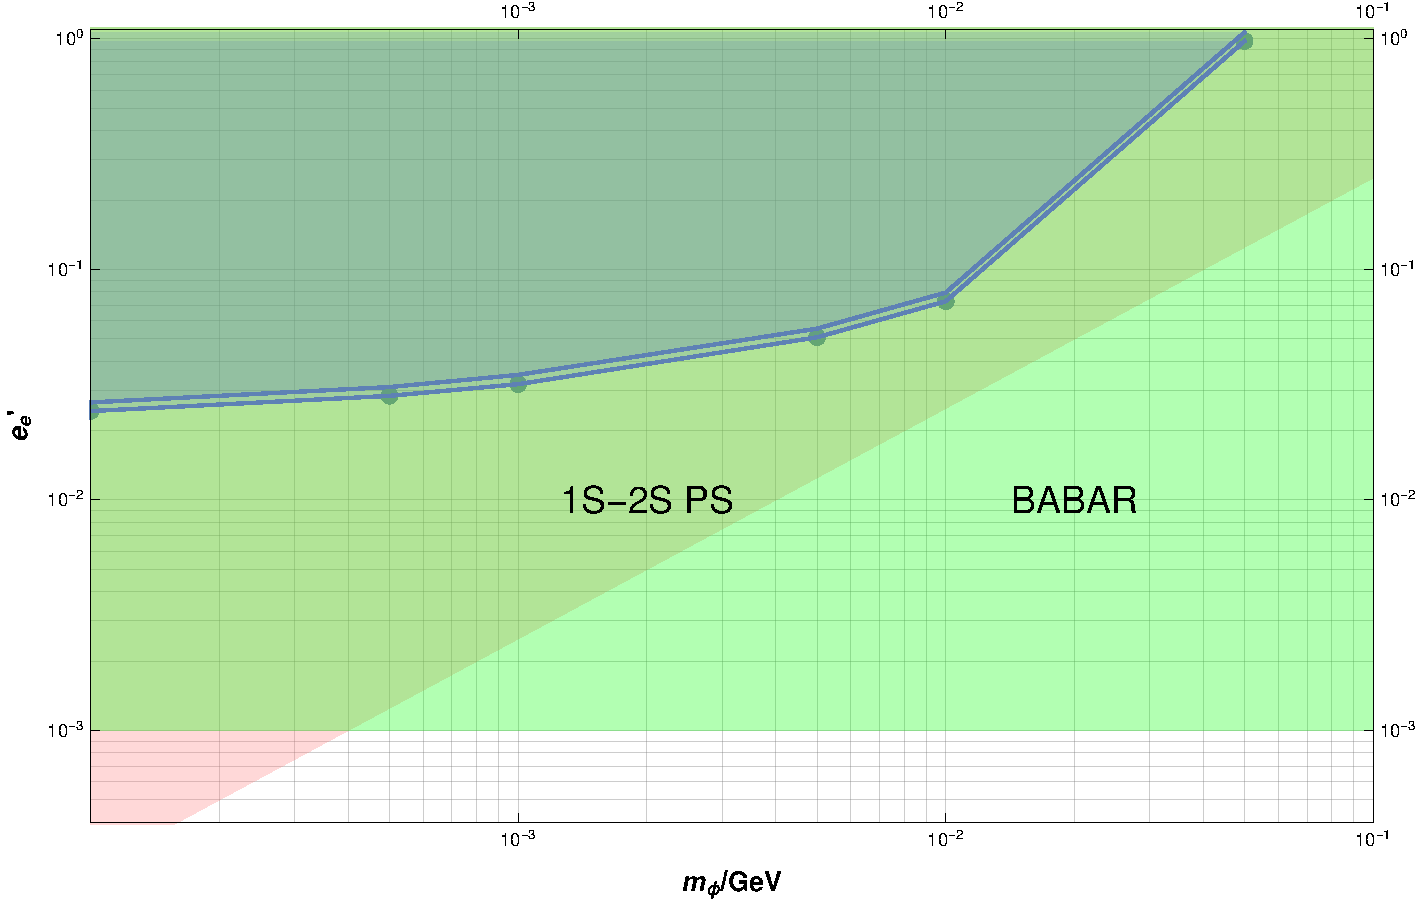
\includegraphics[width=0.8\textwidth]{imgs/MuBoundOnScalarElectron.pdf}
    \caption{90\% and 95\% C.L. bounds on the scalar-electron coupling (blue) with existing bounds from 1S-2S transitions in positronium (brown 95\% C.L.) and missing energy searches by BABAR (green, 95\%C.L.) \cite{Essig:2013vha}}
    \label{fg:MuBoundScEl}
\end{figure}
Shown in figure \ref{fg:MuBoundScEl} are the bound on the coupling between the electron and a scalar mediator. 

\begin{figure}[!ht]
  \centering
    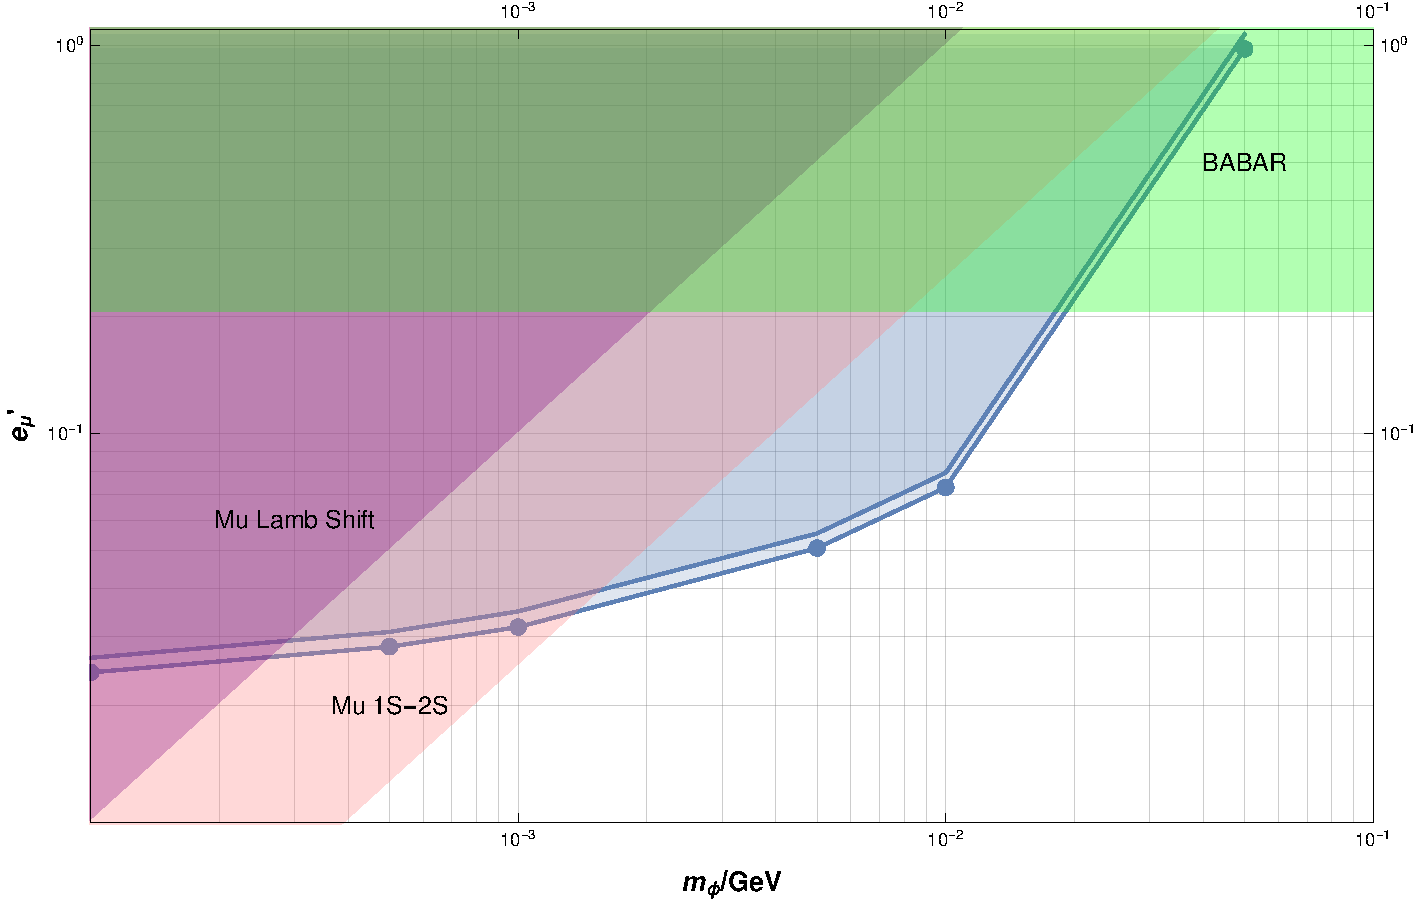
\includegraphics[width=0.8\textwidth]{imgs/MuBoundOnScalarMuon.pdf}
    \caption{90\% and 95\% C.L. bounds on the scalar-muon coupling (blue) and existing bounds for a hierarchical coupling to both lepton families from the Lamb-shift and 1S-2S transition in muonium (purple and red respectively, 95\% C.L.)}
    \label{fg:MuBoundScMu}
\end{figure}
Figure \ref{fg:MuBoundScMu} shows the bounds for the coupling between the muon alone and the scalar mediator that are only slightly stronger than the electron case. This model specifically has not been constrained without further assumptions. Here it is compared to a somewhat better motivated model with mass-hierarchical couplings $e_e'/e_\mu'=m_e/m_\mu$. With this assumption bounds on the product of the couplings $e_e'\times e_\mu'$ from lamb shifts and 1S-2S transitions in muonium can be converted to bounds on the scalar-muon coupling $e_\mu' = \sqrt{e_e'\times e_\mu'\cdot m_\mu/m_e}$. These again have already ruled out most of the parameter space that can be excluded with the muon spectrum. 
\subsection{Vector Mediator}

\begin{figure}[H]
  \centering
    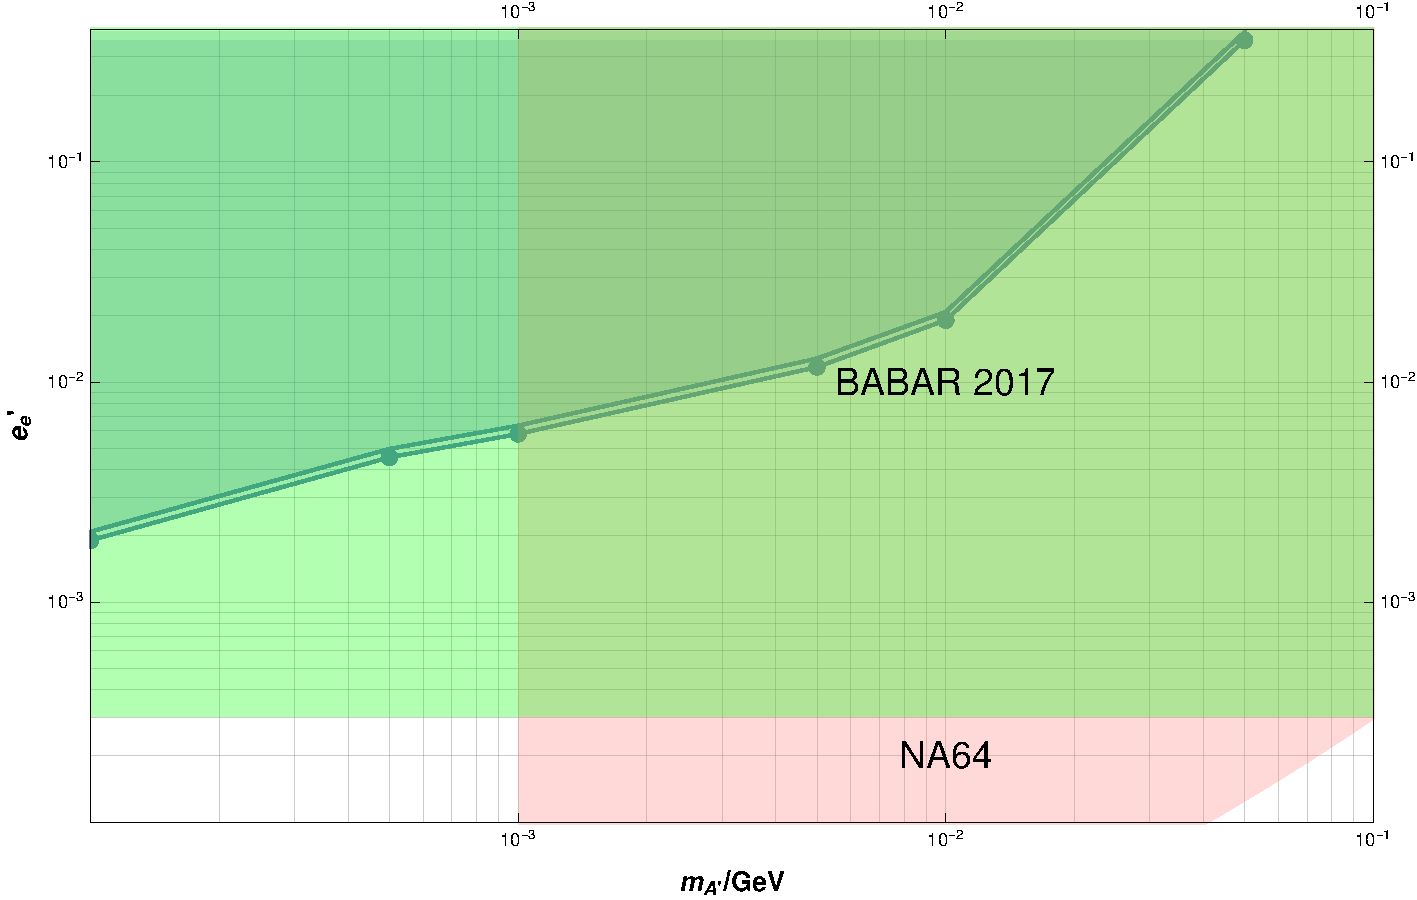
\includegraphics[width=0.8\textwidth]{imgs/MuBoundOnVectorElectron.pdf}
    \caption{90\% and 95\% C.L. bounds on the vector-electron coupling (blue) with existing bounds by NA64 (red 90\% C.L.) and BABAR (green 90\% C.L.)}
    \label{fg:MuBoundVeEl}
\end{figure}
Figure \ref{fg:MuBoundVeEl} shows the bounds on the coupling constants between the muon and a vector mediator alone. The parameter space that could be ruled out with the muon decay has already been constrained by missing energy searches by BABAR and NA64 although the NA64 bounds are only applicable for $m_{A'}>\SI{1}{\mega \eV}$.

\begin{figure}[H]
  \centering
    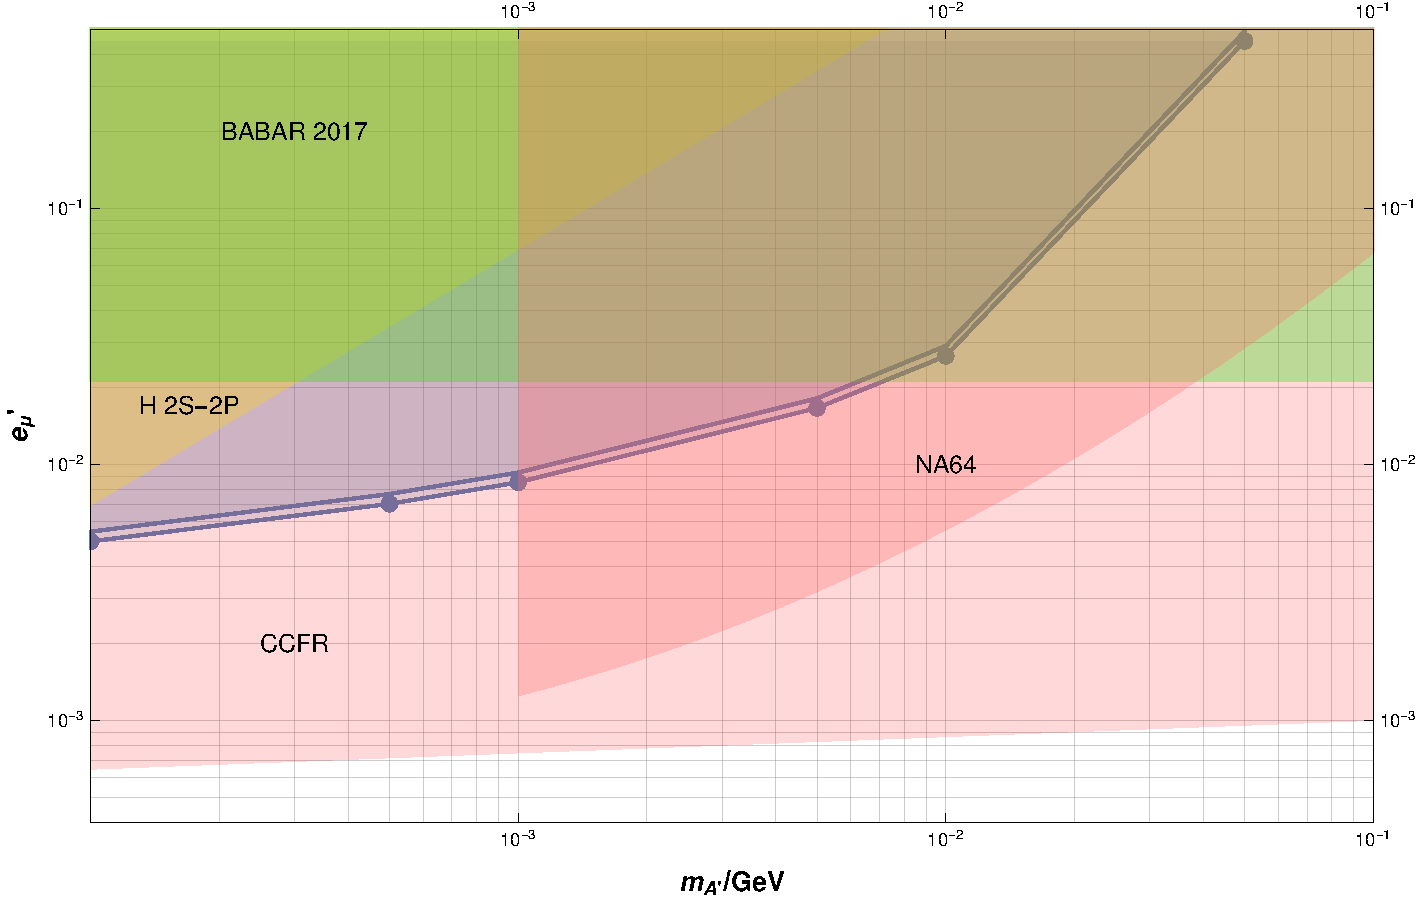
\includegraphics[width=0.8\textwidth]{imgs/MuBoundOnVectorMuon.pdf}
    \caption{90\% and 95\% C.L. bounds on the vector-muon coupling (blue) with existing bounds for the specific $L_{\mu-\tau}$ model by NA64 (red 90\% C.L.) and BABAR (green 90\% C.L.) and hydrogen 2S-2P transition (yellow 95\% C.L.) and neutrino trident production from CCFR (light pink 95\% C.L.)}
    \label{fg:MuBoundVeMu}
\end{figure}
Figure \ref{fg:MuBoundVeMu} shows bounds from the muon decay with only a direct coupling between the muon and the vector mediator. Again since the model with direct coupling only to one lepton family contains anomalies and isn't well motivated there are few existing bounds besides from neutrino trident production shown in the graph. Out of the anomaly free models with gauged $L_{B-L},L_{e-\mu}$ or $L_{\mu-\tau}$ the latter will result in the weakest existing bounds. The resulting expression for the 1-loop kinetic mixing can then be used to translate the existing bounds on the kinetic mixing parameter $\epsilon$ from the NA64 and BABAR experiments to bounds on $e_\mu'$ shown. Additionally to these bounds from hydrogen 2S-2P transitions are used. 
\begin{figure}[H]
  \centering
    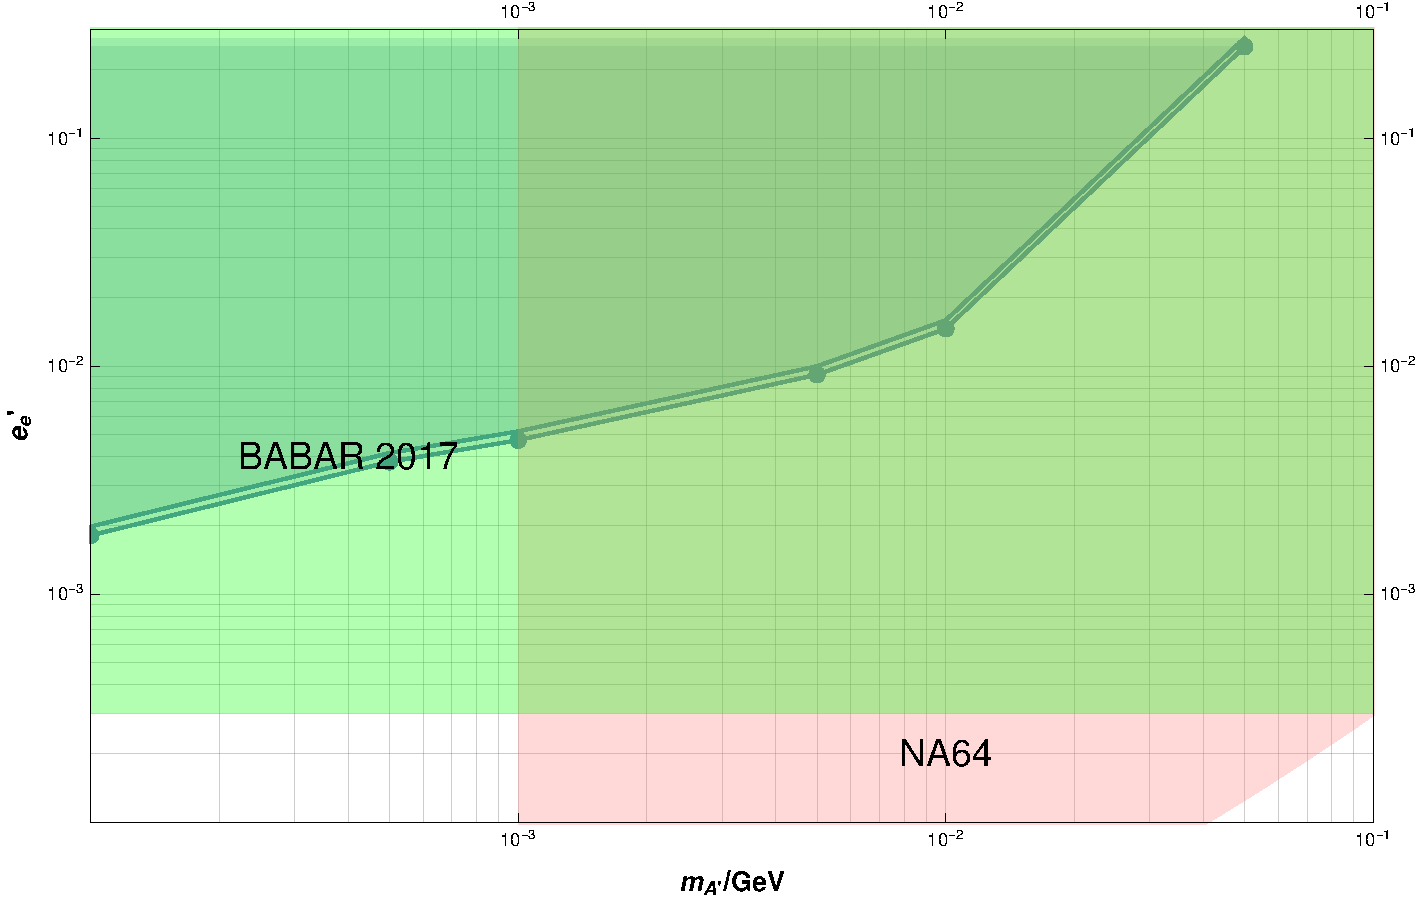
\includegraphics[width=0.8\textwidth]{imgs/MuBoundOnVectorLepton.pdf}
    \caption{90\% and 95\% C.L. bounds on the vector-lepton ($e_e'=-e_\mu'$) coupling (blue) with existing bounds by NA64 (red 90\% C.L.) and BABAR (green 90\% C.L.)}
    \label{fg:MuBoundVeEM}
\end{figure}

Lastly figure \ref{fg:MuBoundVeEM} shows bounds for the model with gauged $L_{e-\mu}$. Here again the bounds from BABAR and NA64 directly apply without further specifications.

\section{Discussion}
The bounds on the electron-scalar coupling obtained here are already ruled out by the BABAR data and the 1S-2S transition in positronium independently. An improvement of the experimental values of the Michel parameters of about three orders is needed to compete with the BABAR result. So this model will not be further constrained using the muon decay in the near future. 

Similar bounds for the muon specific scalar interaction has not been considered in the literature. These results can be compared to to the mass hierarchical coupling between the scalar and the standard model leptons. This way the muon results are related to the electron coupling bounds, though considerably weaker. Additionally results from muonium spectrography become applicable. Compared to these constraints, the ones from the muon decay exclude an additional section of parameter space for mediator masses between 2 and \SI{20}{\mega \eV}.

The constraints on the coupling between the vector mediator and the electron are again much weaker than those obtained by BABAR. Below a mediator mass of \SI{1}{\mega \eV} the uncertainties of the Michel parameters have to be improves only by two orders. NA64 becomes applicable above \SI{1}{\mega \eV} so even a great precision improvement in the muon decay will not become competitive here.

The coupling between the muon and the vector mediator will again need more care. Here the gauged $L_{\mu-\tau}$ model is chosen for comparison. Since this lacks a tree-level coupling to the electron it avoids the generally strong constraints but can nevertheless be implemented anomaly free. Here the kinetic mixing
\begin{equation}
\epsilon = \frac{ee'_\mu}{12\pi^2}\ln\left(\frac{m_\tau^2}{m_\mu^2}\right)
\end{equation}
with $e'_\mu=-e'_\tau$ is used to convert bounds on $\epsilon$ or even to the electron alone to constraints on $e'_\mu$. The results from BABAR alone are in this case weaker than the muon decay results. With the inclusion of the NA64 results no new constraints could be derived for mediator masses above \SI{1}{\mega\eV}. Below the neutrino trident production results from CCFR are used for comparison. Since these apply directly at tree-level without a loop, it results in stronger constraints that already ruled out the results from the muon spectrum. Also shown is the bound from 2S-2P transitions in hydrogen. 

The last considered model with gauged $L_{e-\mu}$ couples to all involved particles. But since it has a tree level coupling to the electron, the BABAR results apply directly and the bounds are not competitive. Here only the bounds on masses below \SI{1}{\mega \eV} will become competitive if the uncertainties are improved by two orders of magnitude. Otherwise an improvement by at least three orders would be needed. This should be well out of reach of experiments in the near future.

A widening of the fiducial region by means of detector improvements will not lead to competitive bounds, even for a perfect detector that is capable to reliably observe the whole spectrum. 